% !TEX root = ../main.tex

\chapter{相关工作}

\section{手势的定义与身体姿态的参数化表示}

\subsection{手势的定义与范围}

在人类交流中,手势(gesture)是与语音同时出现的重要非语言信号,它承担语义补充、情感表达与互动调节等多重功能。McNeill(1992)\cite{mcneill_1992_hand}提出,手势并非语言的附属物,而是语言思维的外化形式,是语音与思维之间的中介过程。Kendon(2004)\cite{kendon_2004_gesture}进一步指出,手势涵盖从手部动作、头部运动到上身姿态的广义身体行为,构成“可见的发话(visible utterance)”。在此框架下,手势与语言并非分离系统,而是同源于共同的认知与表达机制。

\paragraph{手部手势的分类}
McNeill(1992)\cite{mcneill_1992_hand} 将随语音共现的手部动作划分为四种基本类型。%
这一体系从认知与语义功能的角度揭示了手势与语言之间的互动关系,%
并构成了当代手势研究与生成建模的重要理论基础。

\begin{enumerate}
  \item \textbf{Iconic gestures(形象性手势)}:以具象方式描绘事物的外形、空间路径或动作特征,例如用手势勾勒一个圆形或表示“上升”的轨迹。此类手势与语言内容直接对应,表达具体语义。
  \item \textbf{Metaphoric gestures(隐喻性手势)}:表达抽象概念或思维结构的手势,%
如用手的展开表示“扩展话题”或“阐述概念”。%
它们并不描绘实体,而是以具象化的方式呈现抽象语义。
  \item \textbf{Deictic gestures(指示性手势)}:指向空间中的对象、人物或方向,常用于对话焦点的指明与注意引导。
  \item \textbf{Beat gestures(节奏型手势)}:与语音重音、韵律或节奏结构同步的节奏性动作,不承载具体语义,但用于强调语音节奏与结构边界。
\end{enumerate}

这四类手势共同构成了语言—动作系统的语义与功能层次。%
在自然交流中,它们往往混合出现,%
而在建模与生成任务中,通常根据可观测特征或任务目标对其进行功能性区分。%

\paragraph{头部手势的分类}
除手部动作外,头部动作同样是人类多模态交流的重要组成部分。%
头部的点动与摆动在时间结构上常与手势及语音节奏保持同步\cite{gesture_and_speech_in_interaction},%
在语用功能上既能辅助语音韵律的组织,也能表达态度与指向信息。%

在不同研究中,头部动作被从多个维度加以分析,%
其主要功能可归纳为以下几方面:%
\begin{enumerate}
  \item \textbf{韵律相关(prosodic)}动作反映语音重音与句法节奏的对应关系\cite{hadar_1989_headmovement};%
  \item \textbf{语义或态度相关(semantic/attitudinal)}动作表达说话者的情绪倾向与交际意图\cite{kendon_2004_gesture,mcneill_1992_hand};%
  \item \textbf{指向相关(deictic)}动作通过转头或注视方向建立叙事空间的参照\cite{mcneill_1992_hand}。
\end{enumerate}

此外,实验语音学研究发现,头部动作的启动时间往往早于韵律词的发声~\cite{esteve2017timing},%
提示其在时间组织上可能具有前瞻性。%
这一特征揭示了头部动作与语音之间的紧密时序耦合,%
说明视觉模态中的运动信号有时可先于声学事件出现,%
反映出多模态交流中的感知与表达的时间分布特性。%

\subsection{身体姿态的参数化表示}
手势作为身体运动的子集,其生成和识别依赖于身体姿态的连续建模。因此,在进一步讨论手势生成方法之前,有必要明确身体姿态的参数化表示方式。

\paragraph{骨架结构的定义}
在计算机动画与动作捕捉领域,身体姿态通常由骨架结构(skeleton hierarchy)和关节旋转参数(joint rotations)共同定义。骨架结构描述了人体各关节的拓扑关系及层级依赖;而每个姿态帧(pose frame)由一组关节旋转参数所确定,这些参数定义了相对于父节点的旋转变换。在不同的系统与任务中,骨架结构的具体形式往往有所差异,这种差异直接影响姿态数据的表示与学习方式。

在不同的系统与任务中,骨架结构可以遵循各自的标准,因此,不同的数据集、3D模型或神经网络往往基于自身定义的关节层级与命名体系进行训练与标注。例如,AMASS数据集\cite{AMASS:2019}采用SMPL拓扑结构\cite{SMPL:2015},BEAT数据集\cite{beatcamn}使用简化上半身骨架。近年来的自动骨骼绑定与骨架归一化方法,通过学习或优化关节对应关系,实现了不同拓扑之间的姿态重定向(pose retargeting)\cite{GleicherRetargetting1998,MartinelliSkeleton-AwareRetargeting2024},从而消除了模型依赖于特定骨架结构的限制。

\paragraph{旋转参数的选取}
在确定骨架结构之后,具体的关节状态可通过多种旋转参数进行描述。
常见的旋转参数表示方法包括:

\begin{enumerate}
\item 欧拉角(Euler Angles):通过三个顺序旋转角表示姿态,直观但存在“万向节锁(gimbal lock)”问题;
\item 四元数(Quaternion):以四维单位向量表示旋转,避免奇异性,但在神经网络训练中不易约束;
\item Axis-Angle:以旋转轴与旋转角度组合的形式表示,参数紧凑但角度不连续;
\item Rot6d\cite{rot6d}:将旋转矩阵前两列展开为六维向量,通过归一化保持正交性,连续性与可学习性兼具。
\end{enumerate}

在计算机图形与实时渲染中,通常采用四元数或旋转矩阵进行骨骼变换与插值,以保证数值稳定性和计算效率。
然而,在深度学习任务中,这些表示在高维空间中存在不连续性或约束难度。近年来的研究表明\cite{rot6d},Rot6d 表示在动作生成与姿态预测任务中具有更好的连续性与可学习性,可显著提升模型的收敛特性与泛化性能。
因此,本文在姿态生成模型中统一使用 Rot6d 表示每个关节的旋转状态,以确保训练阶段的平滑收敛与推理阶段的稳定性。

不同的手势生成方法在旋转参数的选取上各不相同,相关实例见表~\ref{fig:rotation_comparison}。

\begin{table}[htbp]
\centering
\caption{不同旋转表示方式的空间连续性与使用示例}
\label{fig:rotation_comparison}
\begin{tabular}{@{}lcccc@{}}
\toprule
\textbf{表示方式} & \textbf{维度} & \textbf{连续性} & \textbf{典型应用场景} & \textbf{使用示例} \\ \midrule
欧拉角 & 3 & 存在万向节锁 & 图形学、传统动画 & CaMN\cite{beatcamn} \\
四元数 & 4 & 连续 & 实时渲染、骨骼动画 & — \\
Axis-Angle & 4 & 角度部分不连续 & 动作预测、生成任务 & DiffSHEG\cite{diffsheg} \\
Rot6d & 6 & 连续 & 深度学习生成模型 & EMAGE\cite{emage} \\ \bottomrule
\end{tabular}
\end{table}

\section{面部表情的定义与参数化表示}

面部表情是非语言交流的重要组成部分,与语音、手势共同传递情感和态度信息。与身体动作不同,面部表情主要由皮肤形变和局部运动构成,无法通过骨骼旋转直接建模,因此需要专门的参数化表示方式。

目前常见的面部状态描述方法主要有两类:

\paragraph{BlendShape 权重模型}
FACS(Facial Action Coding System)\cite{EkmanFriesenFACS1978} 提出复杂表情可分解为若干可组合的基本动作单元(Action Units, AU),为表情的参数化表示提供了理论基础。
受此启发,BlendShape 模型将面部表情表示为一组可线性叠加的形变基(morph targets),每个基形对应一个权重控制的局部表情变化。复杂表情由多个基形的组合生成,其思想与 FACS 的动作单元体系相呼应。

与基于骨骼的形变不同,BlendShape 直接在顶点层面定义几何偏移量,因此对网格拓扑结构高度依赖:每个基形的顶点偏移需与基础网格逐点对应。在具有相同网格结构的角色模型之间,BlendShape 集合可以直接复用;但若拓扑(如顶点数量、索引或连线关系)发生变化,偏移数据将无法一一对应,从而难以在不同模型间映射或重定向。这种拓扑依赖性限制了其跨模型的通用性。

尽管如此,BlendShape 在表现精细面部表情和软组织形变方面具有显著优势。其标准化权重接口、实时可驱动性与渲染兼容性,使其成为虚拟人和表情捕捉系统的主流表示形式,并被广泛应用于如 ARKit \cite{ARKitDocumentation} 等实时动画框架,以及主流渲染引擎中。

\begin{figure}[h!t]
\centering
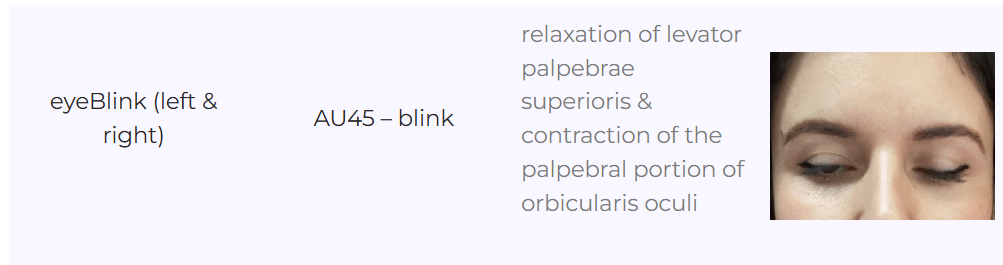
\includegraphics[width=0.95\linewidth]{figures/Fig_AUSample.png}
\caption{示例图来自~\cite{ozel_arkit_facs_cheatsheet},展示 FACS AU45(blink)对应的 ARKit 中的两种 BlendShape 基形:\texttt{eyeBlinkLeft}(闭左眼)与 \texttt{eyeBlinkRight}(闭右眼)。}
\label{fig:au_sample}
\end{figure}

图~\ref{fig:bs_eyeblink} 展示了 \texttt{eyeBlinkLeft}、\texttt{eyeBlinkRight} 的ARKit BlendShape基形在权重 $w\!\in\![0,1]$ 下的线性插值效果(从张眼到闭眼)。

\begin{figure}[h!t]
\centering
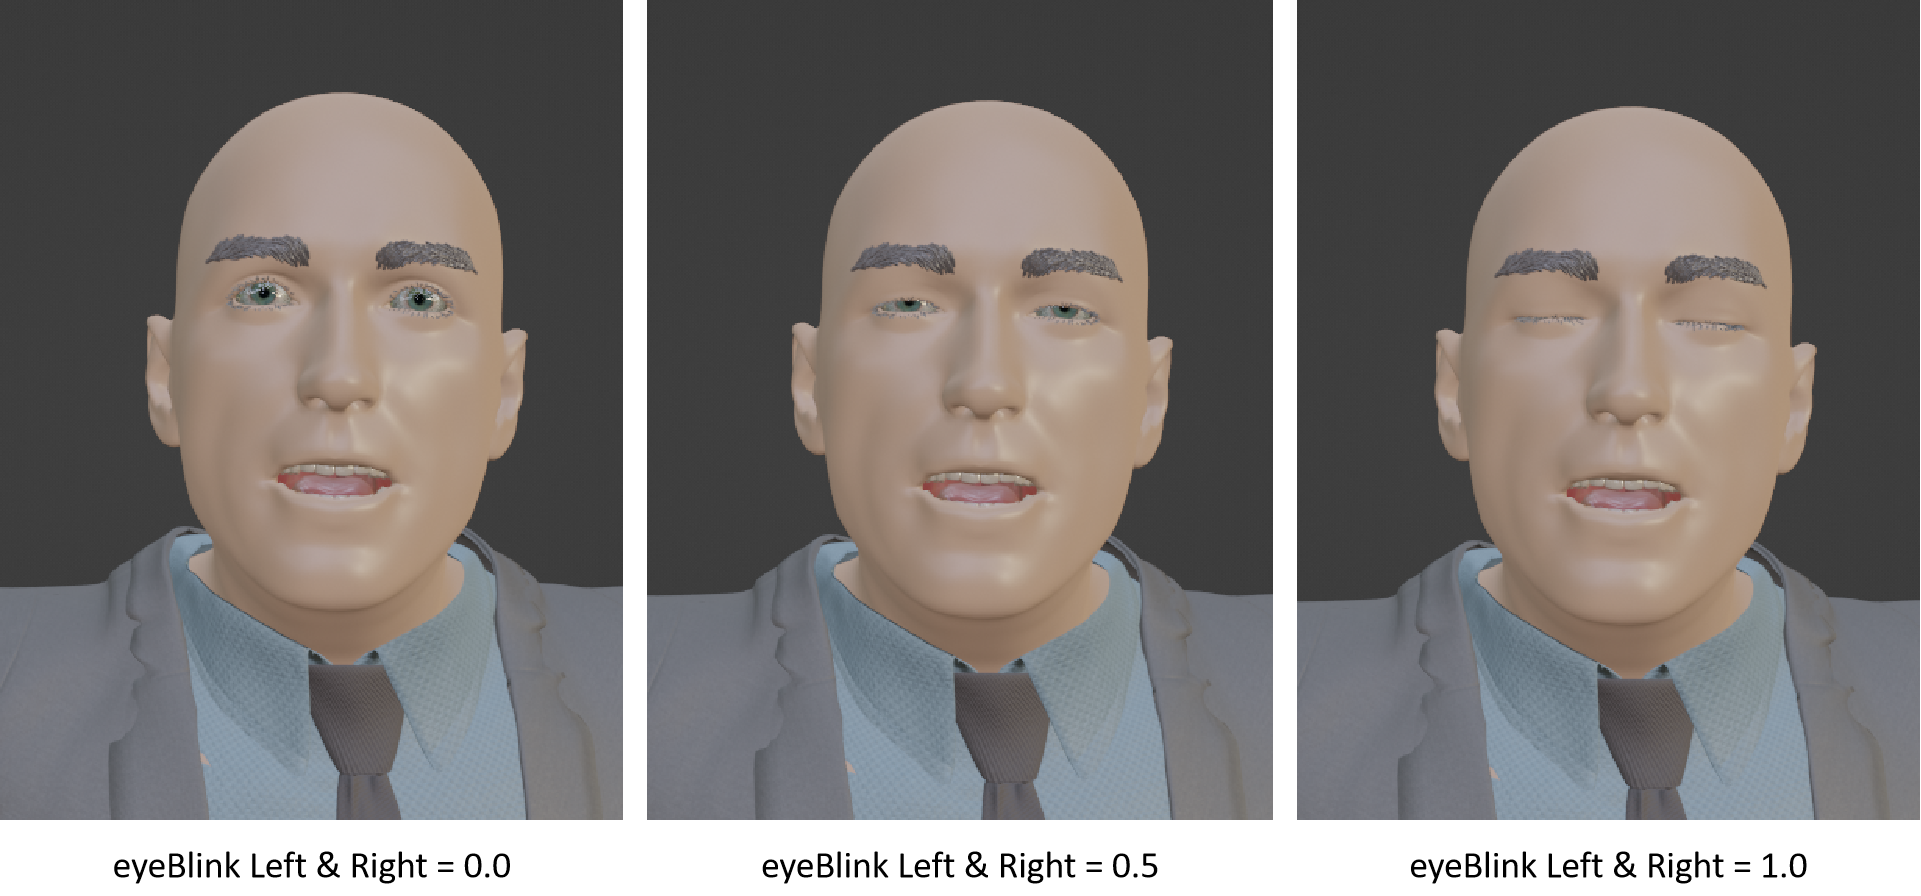
\includegraphics[width=0.95\linewidth]{figures/Fig_blendshapeEyeBlink.png}
\caption{BlendShape 线性插值效果示例:\texttt{eyeBlink} 从 $w{=}0$(左)到 $w{=}1$(右)的连续变化,中图为中间值。BS 权重可直接用于实时渲染驱动。}
\label{fig:bs_eyeblink}
\end{figure}

\paragraph{关键点坐标模型(Landmark-based Representation)}
关键点模型通过检测面部若干语义特征点(2D 或 3D 坐标)来描述几何结构变化。典型实现包括 MediaPipe Face Mesh \cite{mediapipefacemesh} 与 OpenFace 系列。

与基于网格形变的 BlendShape 不同,关键点模型并不依附于任何具体网格拓扑,而是在几何空间中以语义一致的特征点集合形式定义面部结构。这种表示方式并不描述模型的形变,而是对“人脸几何”的抽象建模,因此常用于表情识别、头部姿态估计等分析任务,而较少用于驱动渲染。

在多模态学习与特征分析中,BlendShape 表示具有较高的统一性和可量化性,适合以固定维度向量作为模型输入,并易于应用于不同虚拟角色的动画驱动。因此,本文在系统设计中采用与 ARKit 兼容的 BlendShape 参数作为面部模态输入特征。

\begin{figure}[h!t]
\centering
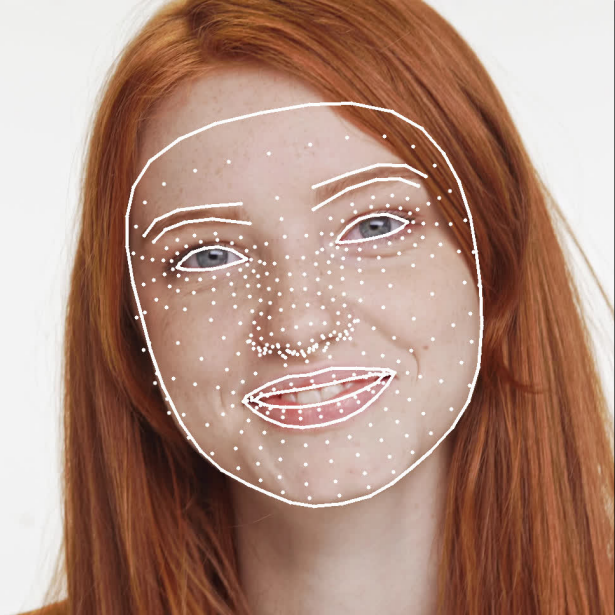
\includegraphics[width=0.4\linewidth]{figures/Fig_MediaPipeLandmark.png}
\caption{MediaPipe Face Mesh 关键点结构示意图,截取自 \cite{mediapipefacemesh}。}
\label{fig_mediapipe_landmark}
\end{figure}

\section{国内外研究现状}

\subsection{手势生成的研究目标}

\subsubsection{研究目标类型的差异}

语音驱动的手势生成研究在总体目标上虽一致——即让虚拟角色的动作与语音内容、节奏协调一致——但在使用场景与系统角色上存在显著差异。

现有研究大体可分为两类:

\paragraph{为AI的虚拟形象生成手势}

这一类研究的目标是让AI驱动的文本对话系统的虚拟形象具备手势表现力。

模型可以一次性生成下一句语音或文本,因此可以访问完整的未来信息,包括整句音频、文本和语义上下文。

典型方法通过编码完整句子的节奏与语义,预测整段动作轨迹,以最大化动作与语义的一致性和整体流畅性。

这类方法适合AI驱动的系统或离线生成的应用场景,如合成视频。

\paragraph{为用户的虚拟人生成实时手势}
本文所聚焦的目标类型属于第二类。

在用户实时说话的过程中,系统需根据当前语音流(以及可选的面部表情与头部姿态)即时生成同步手势。

此任务具有严格的实时性约束与因果性限制:模型在每一时刻只能使用当前及过去的信息,而不能访问未来语音或文本内容。

因此,常见的整句式规划或滑动预测方法不再适用。

该任务更接近实时交互系统,而非内容生成系统。

\subsubsection{任务约束与可利用条件的差异}

这两类研究目标在可利用的信息条件和评价重心上存在本质区别:

\begin{table}[h]
\centering
\caption{两类手势生成任务在约束与可利用条件上的对比}
\label{tab:task_constraint_comparison}
\begin{tabular}{@{}p{3cm}p{5.5cm}p{5.5cm}@{}}
\toprule
\textbf{对比维度} & \textbf{AI 虚拟形象生成} & \textbf{用户虚拟人实时生成} \\ 
\midrule
输入信息 & 完整句级语音或文本(可使用未来信息) & 实时语音流,仅使用过去与当前帧 \\ 
输出目标 & 整句手势序列(离线生成) & 连续流式手势(逐帧生成) \\ 
时间约束 & 不必要实时 & 帧级实时性($<$50\,ms 推理延迟) \\ 
评价重点 & 整体语义一致性与美学自然度 & 瞬时同步性、动作平滑与交互稳定性 \\ 
应用场景 & 离线动画、内容合成、AI虚拟直播 & 实时虚拟人、视频会议、用户虚拟直播 \\ 
\midrule
语音模态 & 作为输入或由文本生成(TTS 输出) & 作为实时输入特征(语音流) \\ 
手部手势 & 生成目标(输出) & 生成目标(输出) \\ 
面部表情 & 通常为生成目标(输出) & 可通过设备实时采集,作为输入辅助推理 \\ 
头部姿态 & 通常为生成目标(输出) & 可实时采集并作为输入特征,用于同步推理 \\ 
\bottomrule
\end{tabular}
\end{table}

前者可以在生成阶段规划动作节奏与语义对应,而后者需在无未来信息的条件下维持自然与同步,
并保证输出连续、平滑且无突跳,从而对模型结构、输入模态与延迟控制提出更高要求。

\subsubsection{评估方法}

语音驱动手势生成研究的评价体系通常涵盖生成质量、时序匹配与表达多样性等多个维度。
研究者既关注生成动作的自然性与视觉流畅度,也重视其与语音信号在节奏和语义层面的对应关系。
近年来,随着实时生成和多模态扩展任务的发展,相关评估方法也逐渐体系化,可概括为以下几类:

\begin{enumerate}
    \item \textbf{自然性(Naturalness)} —— 衡量生成动作在运动平滑性、速度变化及能量分布上的合理性,常采用 FGD(Fréchet Gesture Distance)\cite{ginosar2019speech2gesture}、
          运动速度统计、或主观“自然度”评分等指标。
    \item \textbf{同步性(Synchronization)} —— 评估手势在时间上与语音重音或韵律事件的对齐程度,
          常用 BA(Beat Alignment)\cite{kucherenko2021predictability}、DTW(Dynamic Time Warping)等方法,
          以及基于重读检测的主观同步性评价。
    \item \textbf{多样性(Diversity)} —— 衡量模型在不同语音输入下生成的动作变化程度,
          通常以轨迹分布的方差、速度曲线差异或 L1DIV 等指标度量,
          以防止模型陷入单一模式或过度平滑。
    \item \textbf{语义相关性(Semantic Relevance)} —— 反映生成动作与语义关键词或情绪类别的一致性,
          可通过 SRGR(Semantic Relevance to Gesture Ratio)\cite{beatcamn} 等指标或人工标注语义标签对齐评估。
    \item \textbf{实时性与稳定性(Latency \& Robustness)} —— 在面向交互系统的研究中,
          还需评估帧级推理延迟与输出平滑性,以确保动作流连续且系统响应及时。
\end{enumerate}

总体而言,现有评价体系既包含客观的运动学与统计指标,也结合主观感知评分,
在不同任务目标下可形成“自然性—同步性—多样性—相关性”的综合评估框架。

\subsection{手势生成的演变}

近年来,语音驱动手势生成经历了从规则设计到数据驱动模型、再到多模态扩展与实时生成的持续演变。
这一过程不仅体现了算法架构的更新,也反映了研究目标与应用场景的变化:
从基于语言规则的行为映射,到学习语音—动作关系的深度生成模型,再到面向交互的多模态实时系统。

\subsubsection{规则驱动阶段}

早期的手势生成系统主要依赖语言学规则与专家知识构建 \cite{behavior_expression_animation_toolkit,robot_behavior_toolkit,gesture_generation_by_imitation,gesture_and_speech_in_interaction}。
这类方法通过语义分类或韵律规则将语音片段映射为预定义的手势模板(如指示、肯定、节奏性动作),并以有限的动作库组合出手势序列。
典型代表如 BEAT toolkit 与 Robot Behavior Toolkit,它们可在虚拟代理或机器人中实现基于语音的同步动作。
然而,手势词典与语法规则的人工设计成本较高,难以覆盖自然语音中的多样变化,导致生成结果缺乏自然性与个体差异。

\subsubsection{数据驱动阶段}

随着大规模语音与动作配对数据的出现,研究者开始采用统计学习和深度神经网络模型学习语音—手势映射关系。
在此阶段,语音通常作为唯一输入模态,模型通过 LSTM、GRU 或 MLP 等结构预测连续手势序列。
典型代表如 CaMN 模型 \cite{beatcamn},其基于 BEAT 数据集 \cite{beatcamn} 训练级联网络,将 LSTM、全连接网络与 GAN 结构相结合,实现从语音到动作的端到端预测。

然而,该类模型多使用欧拉角或离散旋转参数作为手势表示,生成结果容易出现抖动与不连续。
后续工作引入更平滑的表示方式,如 Rot6d \cite{rot6d,emage,AMUSE2024} 或 Axis-Angle \cite{diffsheg},显著提升了动作流畅性。
与此同时,为解决语音与手势间的多对多映射问题,研究者引入了 VQ-VAE \cite{emage,zhang2024SemanticGesticulator} 与扩散模型 \cite{tamingDiffgesture,diffsheg,diffstylegesture,DiffTED2024,diffusion-self-supervised2023},
在保持自然性的同时提升了生成多样性与表现力。

尽管这些方法在客观指标与视觉效果上均优于传统模型,但它们普遍假设可访问完整语音或文本上下文,
属于“整句式(non-streaming)”生成,推理延迟较高,不适用于实时应用。
即便是推理效率较高的模型(如 CaMN、DiffSHEG),也因上下文缓冲机制而引入明显延迟。

\subsubsection{多模态扩展阶段}

为进一步提升动作表现力与语音理解能力,部分研究引入视觉模态或语言语义特征。
例如,CaMN \cite{beatcamn} 在语音输入的基础上融合面部捕捉信息以增强表现;
EMAGE \cite{emage} 与 DiffSHEG \cite{diffsheg} 同时生成手势与面部动作;
DiffTED \cite{DiffTED2024} 实现了端到端的视频合成。

这些多模态生成方法在提升虚拟智能体的自然感与沉浸感方面表现优异,但其任务假设仍基于整句输入,因此主要用于AI 虚拟形象生成或离线内容创作场景,而非实时用户交互。

\subsection{当代生成研究的策略趋势}
近年来的研究主要呈现以下两类技术趋势:

\begin{enumerate}
  \item \textbf{扩散模型与高保真生成(Diffusion-based generation)}:
  近年来扩散模型在手势生成任务中表现出卓越的动作自然度与多样性\cite{diffsheg,diffstylegesture,DiffTED2024,tamingDiffgesture,alexanderson2023diffgesture}。
  这类模型通常以完整语音或文本片段为条件,%
  在多阶段去噪过程中逐步生成高保真手势序列。
  然而,其生成过程依赖未来信息与整句上下文,
  因此主要用于离线生成或虚拟形象合成。
  本文的研究目标与之互补,%
  聚焦于在实时约束下实现低延迟、因果一致的动作生成。%

  \item \textbf{语义增强方向(Semantic-aware generation)}:部分研究尝试通过语义或文本特征扩展生成范围,以覆盖 \emph{iconic} 或 \emph{metaphoric} 手势。
  例如,Yoon 等(2020)\cite{yoon2020speechgesturebert} 将语音与文本嵌入结合,
  Alexanderson 等(2023)\cite{alexanderson2023diffgesture} 引入上下文风格控制,实现了语义相关的动作变化。
  这一方向旨在增强生成结果的语义一致性与表现力,%
  与本文关注的实时性问题互为补充:%
  前者通过丰富输入语义扩展表达范围,%
  而本文则探索在严格因果条件下通过多模态信号增强空间与时间表达。
\end{enumerate}

\section{实时生成的理论基础与可行性分析}
从生成可行性的角度,现有研究普遍认为 \emph{beat} 手势可在无语义理解的条件下由语音韵律直接驱动生成。
大量语音驱动手势研究证实,仅凭语音的能量、时长与音高变化即可合成自然的节奏性上肢动作\cite{ginosar2019speech2gesture,alexanderson2020stylegestures,kucherenko2021movingfastslow}。
这些研究所生成的动作在时间结构上与语音重音同步,体现了语音与手势共享的时间规划机制。

相比之下,\emph{iconic}(形象性)、\emph{metaphoric}(隐喻性)与 \emph{deictic}(指向性)手势均依赖语义或指向关系,需要对话语境或文本语义输入,
难以在严格实时的因果条件下生成。Kucherenko 等\cite{kucherenko2021predictability} 的可预测性分析进一步验证了这一点:
他们发现手势的语义类别和空间指向性在语音特征中几乎不可预测,即便结合文本特征,预测性能也相当有限,
而节奏阶段(phase)相关特征在音频中则具有显著更高的可预测性。
这表明,在缺乏未来语义与全局上下文的实时场景中,仅凭语音模态,模型只能稳定生成节奏层面的动作。

为突破这一限制,本文引入头部姿态模态作为补充输入信号。头部姿态能在实时因果条件下提供部分空间与时间线索:其转头与注视方向反映互动焦点,点头与抬头与语音重读共现,能够在不依赖未来语义信息的前提下,为手势生成提供弱先验约束。
这种模态扩展为实时系统提供了理论上的可行性基础,使模型能够在语音之外获得关于节奏、方向与视角的附加信息。

\paragraph{头部姿态对手势预测的贡献}
头部动作在自然语音中常呈现出一定的时间前瞻性~\cite{esteve2017timing}:%
其启动往往早于对应韵律词的发声,%
这意味着视觉模态可能比声学信号更早反映语音节奏的变化趋势。%
这种时序特性为实时生成任务提供了潜在的预测窗口,%
使系统能够在语音节奏变化尚未显现前,就提前捕获相关的动态线索。%
因此,头部姿态在实时生成中不仅提供同步参考,也可能在时间上形成前驱信号,为手势节奏的自然启动提供时序优势。%

\paragraph{头部姿态对空间锚定与视角一致性的贡献}
头部姿态模态为实时语音驱动的手势生成提供了关键的空间参照信号。%
其与语音韵律在时间组织上高度耦合。%
即使在无未来语义信息的条件下,头部的转向与注视变化仍能反映说话者的注意焦点与叙述方向,%
从而帮助模型在动作生成中保持空间的连贯性与方向一致性。%
这一机制使系统能够在时间与空间两个维度上同步对齐语音与动作,%
让生成的手势在视觉上更具互动感与表达意图。

在 McNeill 的四类手势体系中,头部姿态的引入主要强化了两类动作的生成:  
(1) 对 beat 手势而言,它为语音重读和节奏段落提供显式的时间协同信号,使手部与头部动作在韵律层面更加一致;  
(2) 对 iconic 手势而言,它在具有路径与方向特征的动作中提供空间参考,使模型能够在叙事空间中更稳定地确定动作的方位与轨迹方向。  
通过这两方面的强化,系统在保持实时性的同时获得了更自然的节奏衔接与空间表达。

与此同时,本文亦明确头部姿态模态的作用边界:其核心优势在于捕捉方向、焦点与时序节奏,而非手型语义或复杂形态描摹等细粒度语义特征。换言之,它主要改善手势的位置、方向与视角依附,而非手势的形状描绘或语义内容。对于依赖抽象语义或外指参照的\emph{metaphoric} 与 \emph{deictic} 手势,仍需语言或上下文模态的补充。

总体而言,头部姿态为实时生成提供了介于韵律与语义之间的关键中层约束。%
其时间上的前瞻性与空间上的指向性共同帮助模型在低延迟条件下保持自然、连贯且空间协调的动作表现,%
从而在因果生成框架内有效拓展了语音驱动手势的可表达范围,并为节奏主导型(beat-like)动作的实时生成提供了结构的支持。

\section{本文的工作与创新点}

本文研究的目标是设计一种能够在实时条件下运行的语音驱动手势生成模型,使用户无需动作捕捉设备或特定硬件,仅通过语音输入即可驱动虚拟人的上肢与头部动作。与以往主要面向离线生成或 AI 虚拟形象生成的研究不同,本文关注的任务场景是“用户实时交互”,因此系统必须在严格因果的条件下运行,即只能利用当前与过去的输入帧信息,无法依赖未来语音或文本内容进行整体规划。

现有的高精度手势生成模型在离线场景中表现优异,特别是基于扩散模型或 VQ-VAE 的方法 \cite{tamingDiffgesture, diffsheg, emage, DiffTED2024}, 能够生成自然、连贯且语义相关的手势序列。然而,这些模型通常需要整句语音或文本作为输入,推理过程依赖未来信息以分析语义结构与节奏特征,  
因此难以直接应用于实时交互系统。在无未来信息约束下,模型必须在信息不完整的情况下进行预测,这会显著影响动作生成的自然性与语义一致性。

为缓解上述问题,本文提出利用用户的面部表情与头部姿态作为辅助输入模态,为手势生成过程提供额外的非语言信号。面部表情能反映说话者的情绪与语气变化,在语义模糊的情况下有助于生成更具情感表达的动作;头部姿态则能反映注意方向与交互焦点,在语音节奏变化时为手势生成提供时序上的参考。  
通过将这两种模态与语音信号联合输入模型,系统能够在实时条件下获得更多上下文线索,从而在保持低延迟的同时提升手势生成的自然度与一致性。

本文以 CaMN 模型 \cite{beatcamn} 为基础进行扩展。CaMN 原为离线级联结构,输入包括语音与面部捕捉特征,输出包含手部与头部姿态。本文首先将其输入机制改写为逐帧输入流形式,并引入新的头部特征分析模块,将头部姿态信号作为独立通道输入至级联网络的末端层,以强化模型的时序响应能力。  
在这一结构下,系统可在实时语音流输入条件下逐帧生成动作输出,实现语音、面部与头部信号的联合驱动。

实验结果表明,本文提出的模型在实时性与动作自然性之间取得良好平衡。在典型的桌面端环境下,单帧推理时间约为1毫秒之内,能够满足实时交互需求;同时在 FGD、BA 与主观评测中表现出与离线模型相近的手势自然度与同步性。由此,本文的方法证明了在严格因果条件下,通过多模态输入融合可以有效提升实时手势生成的表现力与稳定性。

\section{本章小结}
本章综述了语音驱动手势生成领域的相关研究现状与发展脉络。  
首先,对手势的概念与在计算机中的参数化表示进行了阐述,说明了手势与面部表情、头部姿态在虚拟人交互中的角色与差异。  
随后,从研究目标的角度分析了不同任务设定之间的区别,指出现有大多数工作聚焦于为 AI 虚拟形象生成整句级动作,而缺乏面向用户实时交互的研究。  
在此基础上,回顾了手势生成方法从规则驱动到数据驱动、从单模态到多模态的演变过程,  
总结了现有模型虽在生成质量上取得显著进展,但在实时性与因果性方面仍存在局限。

最后,结合本文的研究目标,提出了面向实时交互的语音驱动手势生成方案。

